\documentclass[specialist, subf, href, colorlinks=true, 12pt, times, mtpro, final]{disser}

\usepackage[utf8x]{inputenc}
\usepackage[english, russian]{babel}
\usepackage[T2A]{fontenc}
\usepackage{amsmath,amsthm,amssymb}
\usepackage {wrapfig}
\usepackage {enumitem}  
\usepackage{graphicx}
\usepackage{wrapfig}
\usepackage{multicol}
\usepackage{mathrsfs}
\usepackage{xcolor}
\usepackage{hyperref}
\usepackage{tikz}
\usepackage{pdfpages}
\usepackage{algorithm}
\usepackage{algpseudocode}


\usetikzlibrary{decorations.pathreplacing}
\usepackage[a4paper, mag=1000, includefoot, left=1.5cm, right=1.5cm, top=1cm, bottom=1cm, headsep=1cm, footskip=1cm]{geometry}
\usepackage{tikz}
\newcommand{\RNumb}[1]{\uppercase\expandafter{\romannumeral #1\relax}}
\usetikzlibrary{graphs}

\theoremstyle{definition}
\newtheorem{defn}{Определение}[section]
\newtheorem{example}{Пример}[section]
\newtheorem{state}{Утверждение}[section]
\newtheorem{theorem}{Теорема}[section]
\newtheorem{lemma}{Лемма}[section]
\newtheorem{axiom}{Аксиома}[section]
\newtheorem{consequence}{Следствие}[section]
\newtheorem{addition}{Примечание}[section]

\definecolor{linkcolor}{HTML}{0000ff} % цвет ссылок
\definecolor{urlcolor}{HTML}{0000ff} % цвет гиперссылок
\hypersetup{pdfstartview=FitH, linkcolor=linkcolor,urlcolor=urlcolor, colorlinks=true}

\begin{document}
\begin{titlepage}
	\begin{center}
		
		Федеральное государственное бюджетное образовательное учреждение высшего образования 
		<<Московский Государственный Университет им.\,М.\,В.\,Ломоносова>>\\
		
		\vspace{9cm}
		Механико-математический факультет
		
		{\bf Конспект лекций по курсу <<Основы механики сплошных сред>>}
		
		\vspace{9cm}
		\begin{flushright}
			{\bfРаботу выполнили студенты 510 группы}\\
		\end{flushright}
		\vspace{1cm}
		
		\normalsize Москва, 2022
	\end{center}
\end{titlepage}

	
\tableofcontents
	
\newpage
\section{Билет 1. Понятие сплошной среды. Лагранжево и эйлерово описание движения сплошной среды. Индивидуальная производная.}
\newpage
\section{Билет 2. Описание деформации. Тензоры Грина и Альманси. Главные оси и главные значения тензоров. Инварианты тензоров.}
\newpage
\section{Билет 3. Вектор перемещения. Связь вектора перемещения и тензоров деформации. Случай малых деформаций. Геометрический смысл компонент. Относительное изменение объема. Уравнение совместности малых деформаций.}
\newpage
\section{Билет 4. Тензор скоростей деформации. Его связь с полем скоростей. Кинематический смысл компонент тензора скоростей деформации. Дивиргенция скорости.}
\newpage
\section{Билет 5. Распределение скоростей в малой окрестности точки сплошной среды (Формула Коши-Гельмгольца). Вектор вихря. Потенциальность течения.}
\newpage
\section{Билет 6. Производная по времени от интеграла по подвижному объему. Уравнение неразрывности в переменных Эйлера и Лагранжа.}
\begin{center}
    \textit{\underline{Закон сохранения массы для индивидуального объема сплошной среды}}
\end{center}

Закон сохранения массы утверждает, что \textbf{масса M любого индивидуального объема сплошной среды постоянна}:
\begin{center}$
M = const
$\end{center}
\textbf{Индивидуальным объемом} называют выделенную часть среды, состоящую из одних и тех же индивидуальных частиц. В механике сплошных сред интерес представляет не столько масса некоторогообъема, сколько распредление массы по объему, которое характеризируется распределением плотности. Определим понятие плотности. Рассмотрим малый объем $\Delta {V}$ с массой $\Delta m$. Средняя плотность этого объема равна:
\begin{center}$
\rho_{ср} = \frac{\Delta m}{\Delta V}
$\end{center}

Плотность $\rho$ в точке среды определяется как предел этого отношения, когда $\Delta V$ стягивается в рассматриваемую точку:
\begin{center}$
\rho = \lim\limits_{\Delta V \to 0} \frac{\Delta m}{\Delta V}
$\end{center}

Масса в объеме $V$ равна:
\begin{center}$
M = \int\limits_V \rho dV
$\end{center}

\textbf{Закон сохранения массы для конечного индивидуального объема сплошной среды $V_{инд}$} гласит:
\begin{center}$
\frac{d}{dt} \int\limits_{V_{инд}(t)} \rho dV = 0
$\end{center}

$V_{инд}(t)$ - индивидуальный, в общем случае, подвижный объем.

\begin{center}
    \textit{\underline{Производная по времени от интеграла по подвижному индивидуальному объему}}
\end{center}
Выведем формулу дифференцирования по времени интеграла по подвижному объему $V(t)$ от некоторой величины $A(x^i, t)$. По определния производной имеем:
\begin{center}$
\frac{d}{dt} \int\limits_{V(t)} A(x^i,t) dV =
\lim\limits_{\Delta t \to 0} \frac{\int\limits_{V(t + \Delta t)} A(x^i,t + \Delta t)dV - \int\limits_{V(t)}A(x^i,t)dV}{\Delta t}
$\end{center}
В правой части вычтем и прибавим одно и то же слагаемое:
\begin{center}$
\int\limits_{V(t + \Delta t)} A(x^i, t)dV
$\end{center}
Тогда получим
\begin{center}$
\frac{d}{dt} \int\limits_{V(t)} A(x^i,t) dV
=\newline
\lim\limits_{\Delta t \to 0} \frac{\int\limits_{V(t + \Delta t)} A(x^i,t + \Delta t)dV - \int\limits_{V(t + \Delta t)}A(x^i,t)dV}{\Delta t}
+
\lim\limits_{\Delta t \to 0} \frac{\int\limits_{V(t + \Delta t)} A(x^i,t)dV - \int\limits_{V(t)}A(x^i,t)dV}{\Delta t}
=\newline
\lim\limits_{\Delta t \to 0}\int\limits_{V(t + \Delta t)} \frac{A(x^i, t + \Delta t) - A(x^i, t)}{\Delta t}dV
+
\lim\limits_{\Delta t \to 0}\frac{1}{\Delta t}\int\limits_{V(t + \Delta t) - V(t)}A(x^i, t)dV
$\end{center}
Первое слагаемое в последней сумме равно:
\begin{center}$
\int\limits_{V(t)}\frac{\partial A}{\partial t}dV
$\end{center}
Для вычисления второго слагаемого разбиваем область $V(t + \Delta t) - V(t)$ на сумму $N$ малых цилиндров с основаниями $\Delta \sigma_k$, представляющими собой элементы поверхности $\Sigma$ объема $V(t)$, и длинами образующих $|\Vec{v}|\Delta
t$. Объем элементарного цилиндра равен произведению площади основания на высоту:
\begin{center}$
\Delta V_k = \Delta \sigma_k v_{n_k} \Delta t,
$\end{center}
где $v_{n_k}$ - проекция скорости на нормаль к площадке $\Delta \sigma_k$. Интеграл по области $V(t + \Delta t) - V(t)$ можно представить как соответсвующий предел суммы произведений значений подинтегральной функции в точках элементарных цилиндров на объемы этих цилиндров. Тогда второе слагаемое вычисляется так:
\begin{center}$
\lim\limits_{\Delta t \to 0} \frac{1}{\Delta t}\lim\limits_{N \to \infty}\sum_{k=1}^{N}A(x_k^i,t)v_{n_k}\Delta t \Delta \sigma_k
=
\int\limits_{\Sigma}Av_n d\sigma
$\end{center}
где $\Sigma$ - поверхность объема V(t)

Итак, \textbf{формула дифференцирования по времени интеграла по подвижному объему} выглядит так:
\begin{equation}
    \frac{d}{dt}\int\limits_{V(t)}A dv= \int\limits_V \frac{\partial A}{\partial t} dV + \int\limits_{\Sigma}A v_n d\sigma
\end{equation}
С использованием формулы (1) \textbf{закон сохранения массы} может быть записан в виде:
\begin{equation}
    \int\limits_V \frac{\partial \rho}{\partial t} dV + \int\limits_{\Sigma}\rho v_n d \sigma = 0
\end{equation}

\begin{center}
    \textit{\underline{Дифференциальное уравнение неразрывности - следствие закона сохранения массы}}
\end{center}
Диффренциальное уравнение, которое выводится из закона сохранения массы, называется \textbf{уравнением неразрывности}. Для вывода уравнения неразрывности нужно преобразовать поверхностный интеграл в соотношении (2) в объемный. Пусть $\rho, \Vec{v}$ непрерывны и дифференцируемы в $V$. Применяем формулу Гаусса-Остроградского. В декартовой системе координат имеем
\begin{center}$
\int\limits_{\Sigma} \rho v_n d \sigma
= \int\limits_{\Sigma} (\rho v_x cos \hat{(n,x)} + \rho v_y cos \hat{(n,y)} + \rho v_z cos \hat{(n,z)})d \sigma
=\newline
\int\limits_V ( \frac{\partial \rho v_x}{\partial x} + \frac{\partial \rho v_y}{\partial y} + \frac{\partial \rho v_z}{\partial z})dV
=
\int\limits_V (div \rho \Vec{v})dV
$\end{center}
Следовительно, для непрерывного движения закон сохранения массы может быть записан в виде:
\begin{center}$
\int\limits_V (\frac{\partial \rho}{\partial t} + div \rho \Vec{v})dV = 0
$\end{center}
Так как это равенство должно выполняться для любого объема, то если подынтегральное выражение непрерывно, то оно должно равняться нулю. Получаем
\textbf{уравнение неразрывности при эйлеровом описании}:
\begin{equation}
    \frac{\partial \rho}{\partial t} + div (\rho \Vec{v}) = 0
\end{equation}
Напомним, что в произвольной системе координат
\begin{center}$
div \rho \Vec{v} = \nabla_i(\rho v^i)
$\end{center}
В декартовых координатах уравнение неразрывности записывается так:
\begin{center}$
\frac{\partial \rho}{\partial t} + \frac{\partial \rho v_x}{\partial x} + \frac{\partial \rho v_y}{\partial y} + \frac{\partial \rho v_z}{\partial z} = 0
$\end{center}
или
\begin{center}$
\frac{\partial \rho}{\partial t} + v_x \frac{\partial \rho}{\partial x} + v_y \frac{\partial \rho}{\partial y} + v_z \frac{\partial \rho}{\partial z} + \rho div (\Vec{v}) = 0
$\end{center}
Полная (ииндивидуальная) производная по времени $\frac{d \rho}{d t}$ определяется формулой
\begin{center}$
\frac{d \rho}{d t} = \frac{\partial \rho}{\partial t} + v_x \frac{\partial \rho}{\partial x} + v_y \frac{\partial \rho}{\partial y} + v_z \frac{\partial \rho}{\partial z}
$\end{center}
поэтому \textbf{уравнение неразрывности} можно записать так:
\begin{equation}
    \frac{d \rho}{d t} + \rho div(\Vec{v}) = 0
\end{equation}
Уравнения (3) и (4) представляют собой две различные формы уравнения неразрывности в эйлеровых переменных.

\begin{center}
    \textit{\underline{Уравнение неразрывности в лагранжевых координатах}}
\end{center}
Уравнение неразрывности следует из закона сохранения массы. В эйлеровых (пространственных) координатах оно имеет вид:
\begin{equation}
    \frac{d \rho}{d t} + \rho div(\Vec{v}) = 0
\end{equation}
где
\begin{center}$
\frac{d \rho}{d t} = \frac{\partial \rho}{\partial t} + v^k \nabla_k \rho,
\nabla_k \rho = \frac{\partial \rho}{\partial x^k}
$\end{center}
В лагранжевых координатах $\xi^i$ индивидуальная производная плотности по времени есть просто частная производная:
\begin{center}$
\frac{d \rho}{d t}  = \frac{\partial \rho (t, \xi)}{\partial t}
$\end{center}
(через $\xi$ обозначен набор $\xi^1$, $\xi^2$, $\xi^3$). Поэтому уравнение (5) записывается в лагранжевых координатах так:
\begin{equation}
    \frac{\partial \rho (t, \xi)}{\partial t} + \rho div(\Vec{v}) = 0
\end{equation}
Это один из видов уравнения неразрывности в лагранжевых координатах.
\newpage
\section{Билет 7. Изменение количества движения конечного объема сплошной среды. Массовые и поверхностные силы. Вектор напряжения. Тензор напряжения. Механический смысл его компонент. Изменение момента количества движения}
\newpage
\section{Билет 8. Дифференциальные уравнения движения сплошной среды и момента количества движения. Симметрия тензора напряжения. Теорема живых сил.}
\newpage
\section{Билет 9. Изменение энергии в конечном объеме сплошной среды (первое начало термодинамики). Работа и внутренняя энергия. Уравнение притока тепла.}
\newpage
\section{Билет 10. Понятие температуры. Теплопроводность. Цикл Карно. Абсолютная температура. КПД цикла Карно. Второе начало термодинамики. Энтропия.}



\begin{center}
	\textit{\underline{Понятие температуры}}
\end{center}

Мы говорим, что тело А имеет большую, чем тело В, температуру ($T_A > T_B$), если при контакте тела А с телом В возникает переход тепловой энергии от тела А к телу В. Понятие температуры не имеет смысла в аналитической механике для систем с небольшим числом степеней свободы. На практике температуру можно приписывать телам, состоящим из большого числа частиц. 

Из молекулярно-кинетической теории известно, что температуру можно рассматривать как величину, пропорциональную средней энергии хаотического теплового движения молекул, приходящуюся на одну степень свободы молекулы.  Температура не иммет смысла для неравновесных систем, в которых не успевает происходить выравнивание (планета).  Обычно рассматривают температуру достаточно малых частей тела и изучают тепловые потоки в теле. Опыт показывает, что во многих практических вопросах часто можно предполагать, что термодинамическое равновесие в малых объемах системы имеет место.  


\begin{center}
	\textit{\underline{Теплопроводность}}
\end{center}

Двухпараметрической средой называется среда, все термо- динамические функции которой зависят только от двух термо- динамических параметров состояния. Если эти два параметра - давление р и плотность $\rho$, то удельная внутренняя энергия такой среды должна выражаться через них: $U = U (p, \rho)$.

Если среда представляет собой идеальную сжимаемую жидкость (гаа), то работа внутренних поверхностных сил, отнесенная к единице массы, имеет вид
$$ \frac{1}{dm}dA_{face}^{(i)} = p\ d\frac{1}{\rho} $$
и уравнение притока тепла в предположении, что $q^{**} = 0$ записывается следующим образом:
$$ dU + p\ d\frac{1}{\rho} = dq^{(e)} $$

В совершенном газе давление, плотность и темцература связаны уравнением Клапейрона:
$$ p = \rho R T $$

R - некоторое постоянное число, называемое газовойпостоянной, различное для разных газов. Уравнение этого типа, связывающее давление, температуру, плотность и, возможно, другие физические характеристики среды, называется уравнением состояния.

Можно ввести ушиверсальную (постоянную для всех газов) газовую постоянную R. и постоянную Больцмана к согласно равенствам
$$ R = \frac{R_0}{M} = \frac{k}{m} $$

Здесь М- - средняя масса одной грамм-молекулы газа, определяемая по формуле
$$ \frac{n}{M} = \frac{n_1}{M_1} + ... + \frac{n_k}{M_k} $$

где k - полное число молекул в данном обьеме смеси,  $n_i$ число молекул, а $M_i$ - соответствующие массы грамм-молекул отдельных сортов газов; m - средняя масса молекулы в граммах.

Совершенный газ можно определить как газ, в котором молекулы взаимодействуют только при столкновениях. Поэтому можно считать, что внутренняя энергия одноатомного соверщенного газа представляет собой суммарную кинетическую ёнергию хаотического движения атомов. 

Для внутренней энергии U единицы массы можно написать
$$ U = \frac{1}{M}\sum\limits_{i=1}^{N}\frac{m_iv_i^2}{2} + const $$

Если считать, что все атомы газа одинаковые, то $M = Nm$ и 
$$ U = \frac{v_{average}^2}{2} + const $$

Для совершенного газа, согласно определению температуры как характеристики средней энергии, приходящейся на одну степень свободы в хаотическом тепловом движении атомов, удельную внутреннюю энергию U можно представить в виде
$$ U = c_VT + const \ \ \ \ (*)$$

Здесь через $c_V$ обозначен размерный коэффициент пропорциональности между $\frac{1}{2}v_{average}^2$ и T

Задание внутренней энергии U в виде $(*)$ вместе с уравнением Клапейрона фиксирует определенную модель сплошной среды, называемую совершенным газом. Сравнения с экспериментальными данными показывают, что движения реальных газов при обычных условиях достаточно хорошо описываются такой моделью.

На основании уравнения притока тепла для совершенного идеального газа в случае процесса, протекающего при постоянном удельном объеме $\left(\displaystyle d\frac{1}{\rho}=0\right)$ можно легко получить, что
$$ (dq^{(e)})_{V = const} = dU = c_VdT $$
или
$$ \left( \frac{dq^{(e)}}{dT} \right)_{V=const} = c_V $$

Следовательно,  $c_V$ представляет собой количество тепла,которое необходимо подвести к единице массы среды для того, чтобы при постоянном объеме поднять ее температуру на $1^oC$;  поэтому $c_V$ называется теплоемкостью при постоянном объеме.

В случае процесса при постоянном давлении из уравнения притока тепла для идеального совершенного газа получим
$$ \left(d q^{(e)}\right)_{p=\text { const }}=d U+p d \frac{1}{\rho}=c_V d T+d \frac{p}{\rho}=\left(c_V+R\right) d T $$

Количество тепла, которое необходимо подвести к единице мас- сы среды, чтобы при постоянном давлении поднять температу- ру на $1^oC$, называется теплоемкостью при постоянном давлении и обозначается через $C_p$:
$$ c_p = \left( \frac{dq^{(e)}}{dT} \right)_{p=const} $$

Следовательно, $$ c_p - c_V = R $$


\begin{center}
	\textit{\underline{Цикл Карно}}
\end{center}

Процесс \textbf{адиабатический}, если в нем отсутствует приток внешнего тепла и теплообмен между соседними частицами. Т.е. $\displaystyle dQ^{(e)} = 0$
Процесс \textbf{изотермический}, если теплообмен, обусловленный теплопроводностью или излучением, пред- ставляет собой настолько интенсивный продесс, а изменение состояний протекает настолько медленно, что температуру всех частей системы можно считать постоянной. Т.е. $\displaystyle \frac{dT}{dt} = 0$

Рассмотрим следующий важный равновесный обратимый замкнутый процесс, который носит название обратимого цикла Карно. Рабочим телом, т. е. средой, которая совершает этот цикл, пусть будет совершенный газ или любая другая двухпараметрическая среда - определяемая параметрами р и $\frac{1}{\rho}$. 

Из произвольной точки $M (p_0, \frac{1}{\rho_0})$ пространства состояний газ по изотерме $\theta_1 = const$ бесконечно медленно расширяется до состояния $N$, затем газ расширяется адиабатически до состояния $K$ с  температурой $\theta_2 < \theta_1$ и от $K$ сжимается изотермически до состояния $P$, из которого можно вновь вернуться по адиабате в первоначальное состояние $M$.

\begin{figure}[H]
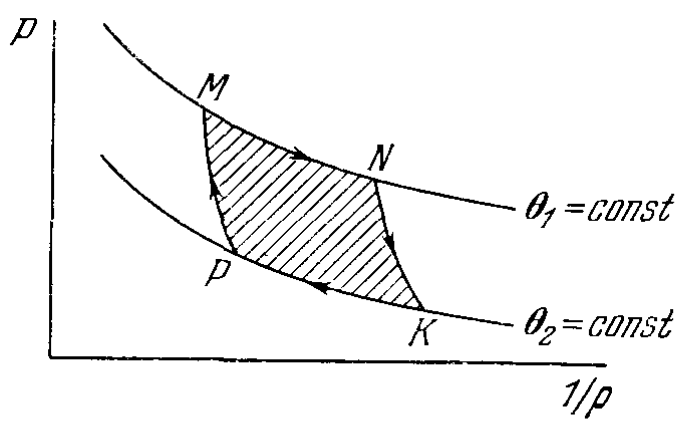
\includegraphics[width=0.7\textwidth]{10/carno.png}
\end{figure}


\begin{center}
	\textit{\underline{Второй закон термодинамики}}
\end{center}

\textbf{Формулировка 1:} Невозможно устройство, которое переводило бы тепло от тела с меньшей температурой к телу с большей температурой без каких-либо изменений в других телах.

\textbf{Формулировка 2:} нельзя построить так называемый вечный двигатель второго рода, т.е. машину,  которая,  работая в согласии с первым законом термодинамики по некоторому циклу,  периодически совершала бы работу только за счет охлаждения некоторого одного и того же источника тепла с фиксированной температурой (отбор тепла из резервуара с постоянной температурой).

$$ A = Q_1 - Q_2 $$

Введем понятие коэффициента полезного действия (к.п.д.) $\eta$ тепловой машины, работающей по циклу Карно. По определению к.п.д.  цикла Карно называется отношение полученной в результате реализации цикла механической работы $А > 0$ к подведенному к системе за время цикла теплу $Q_1 > 0$.  Для к. п. д. цикла Карно верна формула
$$ \eta = \frac{A}{Q_1} = 1 - \frac{Q_2}{Q_1} < 1 $$

Полученной свойство $\eta < 1$ есть следствие первого закона термодинамики. 

\begin{statement}
	Для всякого обратимого цикла Карно величина $\eta$ зависит только от температур $\theta_1$ и $\theta_2$,  заданных на изотермах $MN$ и $KP$ и не зависит ни от свойств рабочего тела, участвующего в цикле Карно ни от способа организации цикла, определяемого, например, размерами рабочего тела и степенью расширения вдоль изотерм.
\end{statement}

Докажем, что $\eta$ зависит только от $\theta_1$ и $\theta_2$ и является абсолютной характеристикой обратимого цикла Карно, т. е. универсальной функцией $\eta(\theta_1, \theta_2)$. Одновременнос этим покажем,  что еслит емпературы $\theta_1$ и $\theta_2$ фиксированы,то к. п. д. $\eta'$ машины,  работающей по необратимому циклу Карно не может быть больше к. п. д.  $\eta$ машины, работающей по соответствующему обратимому циклу Карно, т. е.
$$ \eta' \leq \eta $$
\begin{proof}
(От противного, противоречие со вторым законом термодинамики):

Пусть есть 2 цикла - обратимый ($\eta$) и необратимый ($\eta'$) c одинаковыми температурами $\theta_1 > \theta_2$. Пусть $\eta' > \eta$. Пусть машина с к.п.д. $\eta'$ работает в прямом направлении и проивзодит работу $A'$. Заставим обратимую машину работать в противоположном направлении (холодильная машина).  Тогда для машины с к.п.д. $\eta'$ имеем $Q'_1 > 0$, $Q'_2 > 0$ и $A' = Q'_1 - Q'_2 > 0$.  А для машины с к.п.д. $\eta$ имеем $Q_1 > 0$, $Q_2 > 0$ и $A = Q_2 - Q_1 < 0$. Выберем обратимый цикл Карно так, чтобы имело место равенство $-A = A'$, т.е. $Q_1' - Q_2' = Q_1 - Q_2$ и соединим эти машины вместе. Получим машину, для которой $$ A_0 = A' + A = Q_1 + Q_2 - Q_1' - Q_2' $$

Единственный эффект, производимый этой составной машиной, будет заключаться в перераспределении теплоты между телами,  которые служат нагревателем и холодильником.

По построению (по выбору машин): $|A| = A' \ \ \Rightarrow \eta Q_1 = \eta'Q_1' $. Значит из предположения $\eta' > \eta$ следует $$ Q_1' < Q_1 $$
или $$ Q_1 - Q_1' = Q_2 - Q_2' > 0 $$
Здесь слева количество тепла,  передаваемое в резервуар с более высокой температурой, а справа - равна общему количеству тепла, забираемому из резервуара с температурой $\theta_2$

Таким образом, составная машина без затраты внешней энергии будет переводить тепло от холодного резервуара к горячему, что невозможно согласно второму закону термодинамики.

\end{proof} 

При доказательстве мы не пользовались ни свойствами рабочего тела ни частными свойствами цикла, следовательно, к.п.д.  обратимого цикла Карно не зависит от свойств рабочего вещества и от степени расширения,  а зависит только от $\theta_1$ и $\theta_2$ и является универсальной функцией $\eta = \eta(\theta_1, \theta_2)$

Найдем эту универсальную функцию.  По определению к.п.д. цикла Карно имеем
$$ \eta(\theta_1, \theta_2) = \frac{A}{Q_1} = 1 - \frac{Q_2}{Q_1} $$
Введем функцию $f(\theta_1, \theta_2) = 1 - \eta(\theta_1, \theta_2) = \frac{Q_2}{Q_1}$

Рассмотрим три тела большой теплоемкости с температурами $\theta_1, \theta_2, \theta_3$ и три обратимых цикла Карно, в которых эти тела служат нагревателями или холодильниками.
$$ f(\theta_1, \theta_2) = \frac{Q_2}{Q_1} = \frac{Q_2}{Q_3}\frac{Q_3}{Q_1} = f(\theta_3, \theta_2)f(\theta_1, \theta_3) $$

В случае $\theta_1 = \theta_2$:
$$ 1 = f(\theta_3, \theta_1)f(\theta_1, \theta_3) $$
То есть при перестановке аргументов функция обращается. Следваотельно, 
$$ \frac{Q_2}{Q_1} = f(\theta_1, \theta_2) = \frac{f(\theta_3, \theta_2)}{f(\theta_3, \theta_1)} \ \ \ \ (**)$$
Отсюда следует, что $\frac{Q_2}{Q_1}$ не зависит от $\theta_3$.  Решение функционального уравнения $(**)$ имеет вид
$$ f(\theta_1, \theta_2) = \frac{\omega(\theta_2)}{\omega(\theta_1)} $$
Следовательно $$ \frac{Q_2}{Q_1} = \frac{\omega(\theta_2)}{\omega(\theta_1)} $$

\begin{definition}
	Абсолютная температура $T$ - значение функции $\omega(\theta)$
\end{definition}

Тогда $$ \frac{Q_2}{Q_1} = \frac{T_2}{T_1} $$

\textbf{Формулировка 3 (количественная для обратимого цикла Карно):} 
$$ \frac{Q_1^{(e)}}{T_1} + \frac{Q_2^{(e)}}{T_2} = 0 $$


\begin{center}
	\textit{\underline{Энтропия}}
\end{center}

Фиксируя точку начального состояния системы А для любого состояния В двупараметрической среды, в которое можно перейти из состояния А обратимыми путями, можно ввести функцию параметров состояния - координат точки В:
$$ S(B) = S\left(p, \frac{1}{\rho}\right) = \int\limits_{A}^{B}\frac{dQ^{(e)}}{T} + S(A) $$

\begin{definition}
	 Энтропия - это функция $S(B)$
\end{definition}

Из определения следует, что $$ dS = \frac{dQ^{(e)}}{T} $$
Из уравнения притока тепла:
$$ dS = \frac{dU_m + dA^{(i)}}{T} $$
Или в рассчете на единицу массы:
$$ ds = \frac{dq^{(e)}}{T} = \frac{dU + pd\frac{1}{\rho}}{T} $$

\textbf{Случай совершенного газа:}

для совершенного газа с постоянными теплоемкостями ($p = \rho R T, \ \ U = c_V T$) будем иметь
$$ ds = \frac{c_VdT}{T} + \frac{Rd\frac{1}{\rho}}{\frac{1}{\rho}} = dln\left[T^{c_V}\left( \frac{1}{\rho} \right)^{R}\right] $$



\newpage
\section{Билет 11. Идеальная жидкость. Уравнения Эйлера. Полная система уравнений, описывающая движения идеальной несжимаемой жидкости. Граничные условия.}

\begin{center} \textit{\underline{Идеальная жидкость}} \end{center}

\begin{defn}[]\textbf{Жидкость} или \textbf{газ} -- это среда, в которой \underline{в состоянии покоя} отсутствуют касательные напряжения, т.е. в состоянии покоя вектор напряжений на любой площадке параллелен нормали к площадке: $ \vec{P_n} || \vec{n} $, то есть $ \vec{P_n} = P_{nn} \vec{n} $, где $ P_{nn} $ -- проекция вектора $ \vec{P_n} $ на нормаль $ \vec{n} $ к площадке.
\end{defn}

\textcolor{gray}{В твёрдом теле это не так. Например, тяжёлый твердый кирпич может лежать на наклонной плоскости. На площадках, параллельных плоскости, действуют касательные силы, которые уравновешивают соответствующую составляющую силы тяжести. Жидкий «кирпич» на наклонной плоскости лежать не может, жидкость будет течь.} 

\begin{theorem}[Э-124] \textbf{Теорема о давлении (закон Паскаля, следствие из ЗСКД или формулы Коши (Э-107))}
Если на всех площадках в данной точке вектор напряжений $ \vec{P_n} $ перпендикулярен площадке, то есть $ \vec{P_n} = P_{nn} \vec{n} $, то величина $ P_{nn} $ на всех площадках в данной точке одна и та же. 
\end{theorem}

Вводится обозначение $P_{nn} = -p$. Величина $p$ называется \textbf{давлением}.

В любой жидкости и любом газе \underline{в состоянии покоя} вектор напряжений имеет вид $ \vec{P_n} = p \vec{n} $, а компоненты тензора напряжений в декартовой СК \underline{в состоянии покоя}: $ p^{ij} = -p \delta^{ij} $.

В движущихся жидкостях и газах, конечно, возникают касательные напряжения.
\textcolor{gray}{Это свойство жидкостей называется вязкостью, а сами касательные напряжения в жидкостях и газах называют вязким трением.}

\begin{defn}[Э-125] Жидкость или газ называются \textbf{идеальными}, если в них не только в состоянии покоя, но и \underline{при движении} отсутствуют касательные напряжения.
\end{defn}

Из определения следует, что компоненты тензора напряжений в декартовой СК для идеальных жидкостей или газа при движении имеют такой же вид, как и в состоянии покоя:
$$ \fbox{ p^{ij} = -p \delta^{ij} } $$

\begin{center} \textit{\underline{Уравнения Эйлера.}} \end{center}

Уравнения движения идеальной жидкости или газа называются \textbf{уравнениями Эйлера}.
Их получают из общих уравнений движения с использованием формулы $ p^{ij} = -p \delta^{ij} $.

Уравнения движения любой среды:
$$ \rho \frac{dv^i}{dt} = \rho F^i + \nabla_k( p^{ik} ) $$

Используем, что в идеальной жидкости:
$$
  p^{ik} = -p \delta^{ik} \;\Rightarrow \;
  \nabla_k( p^{ik} ) = \frac{\partial p^{ik} }{\partial x^k} =
  \delta^{ik} \frac{\partial p }{\partial x^k} = \frac{\partial p }{\partial x^i}
$$

Тогда:
$$ \rho \frac{dv^i}{dt} = \rho F^i + \frac{\partial p }{\partial x^i} $$

\begin{theorem}[Э-126]Уравнения Эйлера:
$$ \fbox{ \rho \frac{d \vec{v}}{dt} = \rho F + \Grad p } $$
\end{theorem}

\begin{center} \textit{\underline{Полная система уравнений, описывающая движения идеальной несжимаемой жидкости.}} \end{center}

\begin{defn}[]Жидкость называется \textbf{несжимаемой}, если её плотность в частице при движении сохраняется.
$$ \rho = \Const \;, \quad \frac{d \rho}{dt} = 0 $$
\end{defn}

Полная система уравнений идеальной жидкости:
$$
\begin{cases}
\frac{d \rho}{dt} = \rho \Div \vec{v} \quad &\text{ --- ур-ние неразрывности } \\
\rho \frac{d \vec{v}}{dt} = \rho F + \Grad p \quad &\text{ --- ур-ние движения }
\end{cases}
$$

Полная система уравнений идеальной \underline{несжимаемой} жидкости (Э-127):
$$
\begin{cases}
\Div \vec{v} = 0 \quad &\text{ --- ур-ние неразрывности } \\
\rho \frac{d \vec{v}}{dt} = \rho F + \Grad p \quad &\text{ --- ур-ние движения }
\end{cases}
$$

\begin{center} \textit{\underline{Граничные условия.}} \end{center}

Границы области, занятой жидкостью, бывают двух типов:
\begin{enumerate}
\item твёрдые, границы тел, погружённых в жидкость (например, стенки трубы, поверхность подводной лодки, движущейся под водой, опоры моста, самолета в воздухе)
\item свободные, форма которых заранее не известна (например, покрытая волнами поверхность моря)
\end{enumerate}

\begin{defn}[Э-128] Граничное условие на поверхности твёрдых тел в идеальной жидкости называется \textbf{условием непроницаемости}. Это условие означает, что жидкость или газ не проникают сквозь эту поверхность.
$$ \left. v_n \right|_{\text{на поверхности тела}} = v_{n тела}$$
где $ v_{n тела} $ -- нормальная составляющая скорости точки поверхности движущегося тела.
\end{defn}


\begin{defn}[Э-128] Граничное условие на поверхности твёрдых тел в идеальной жидкости называется \textbf{условием непроницаемости}. Это условие означает, что жидкость или газ не проникают внутрь тела и не отрывается от него.
Для этого необходимо, чтобы скорости жидкости и соответствующей точки тела вдоль нормали к поверхности тела были одинаковы, то есть в точках поверхности тела выполнялось равенство:
$$ \left. v_n \right|_{\text{на поверхности тела}} = v_{n тела}$$
где $ v_{n тела} $ -- нормальная составляющая скорости точки поверхности движущегося тела.
\end{defn}

Если тело неподвижно, то условие непроницаемости на его поверхности имеет вид:
$$ \left. v_n \right|_{\text{на поверхности тела}} = 0 $$
\newpage
\section{Билет 12. Уравнения движения идеальной жидкости в форме Громеки-Лемба. Интегралы Бернулли и Коши- Лагранжа.}
\newpage
\section{Билет 13. Теоремы о вихрях в идеальной жидкости.}
\newpage
\section{Билет 14. Безвихревое движение идеальной жидкости в трехмерном и в двумерном случаях. Примеры потенциалов. Применение теории функции комплексного переменного для решения задач плоского движения идеальной несжимаемой жидкости. Формула Жуковского.}
\newpage
\section{Билет 15. Совершенный газ. Адиабатический процесс. Полная система уравнений, описывающая движение нетеплопроводного идеального газа. Скорость звука. Число Маха. Критерий сжимаемости в стационарном случае. Квазиодномерные стационарные течения. Сопло Лаваля}
\newpage
\section{Билет 16. Вязкая жидкость. Закон Навье-Стокса. Уравнения Навье-Стокса. Полная система уравнения, описывающая движение вязкой несжимаемой жидкости. Течение Пуазейля. Течение Куэтта. Закон Фурье. Полная система уравнений, описывающая движение вязкого теплопроводного совершенного газа.}
\newpage
\section{Билет 17. Безразмерные параметры, определяющие характер движения несжимаемой вязкой жидкости. Число Рейнольдса. Предельные случаи. Пограничный слой.}
\newpage
\section{Билет 18. Линейно упругое тело. Модуль Юнга, коэффициент Пуассона, коэффициненты Ламе. Связь этих коэффициентов между собой. Их физический смысл. Уравнения Ламе.}
\newpage
\section{Билет 19. Постановка задач теории упругости в перемещениях и напряжениях. Граничные условия. Принцип Сен-Венана.}
\newpage
\section{Билет 20. Задача об изгибе балки.}
\newpage
\section{Билет 21. Кручение цилиндрических стержней}

\newpage
\begin{thebibliography}{100}
	
\end{thebibliography}

\end{document}
